\chapter{Technical Background}
\label{ch:background}

\section{Blood Pressure and Its Clinical Measurement}

Blood pressure (BP) is the force exerted by circulating blood on the walls of the arteries. It is reported as two values: systolic blood pressure (SBP), the maximum pressure during ventricular contraction, and diastolic blood pressure (DBP), the minimum pressure during ventricular relaxation. Hypertension --- persistently elevated BP --- is the leading modifiable risk factor for cardiovascular disease and premature mortality worldwide \citep{allen2007}. Because hypertension is largely asymptomatic, continuous and convenient measurement is essential for early detection and long-term management.

For over a century, the clinical standard for BP measurement has been the inflatable cuff sphygmomanometer. The auscultatory method, introduced by Korotkoff, detects SBP and DBP from the appearance and disappearance of Korotkoff sounds during cuff deflation, while modern automated devices use the oscillometric method, which analyses pressure oscillations in the cuff \citep{bhs1993}. These devices are accurate but inherently intermittent: each measurement requires inflating a cuff, which is inconvenient for frequent use and cannot capture the continuous fluctuations of BP that occur throughout the day and during sleep.

The accuracy of BP devices is assessed against standardised protocols. The British Hypertension Society (BHS) protocol grades devices by the cumulative percentage of readings within 5, 10, and 15 mmHg of the reference \citep{bhs1993}; the IEEE 1708 standard provides a comparable framework for wearable cuffless devices \citep{ieee1708}. These protocols define the clinical-grade accuracy that a cuffless solution must ultimately achieve.

\section{Photoplethysmography}

Photoplethysmography (PPG) is a non-invasive optical technique that measures blood-volume changes in the microvascular bed of the tissue. A light-emitting diode illuminates the skin, and a photodetector measures the transmitted or reflected light; because haemoglobin absorbs light, the detected signal varies with the pulsatile blood volume in each cardiac cycle \citep{allen2007}. This is the same sensing principle used in pulse oximeters for oxygen saturation and in smartwatches for heart-rate monitoring, making PPG the most practical candidate for ambulatory BP estimation.

A PPG waveform mirrors the cardiac cycle and contains a systolic peak, a dicrotic notch, and a diastolic phase. The dicrotic notch corresponds to aortic valve closure, and its prominence reflects vascular tone and arterial stiffness \citep{allen2007}. Because the waveform shape is influenced by arterial compliance, vascular resistance, and cardiac contractility, morphological features extracted from PPG can encode the physiological determinants of BP. Figure~\ref{fig:abp_ppg} contrasts the invasive arterial blood pressure (ABP) waveform with the optical PPG waveform; although they differ in sensing principle and units, they share the same cardiac morphology, which is the basis for using PPG features to estimate BP.

\begin{figure}[htbp]
\centering
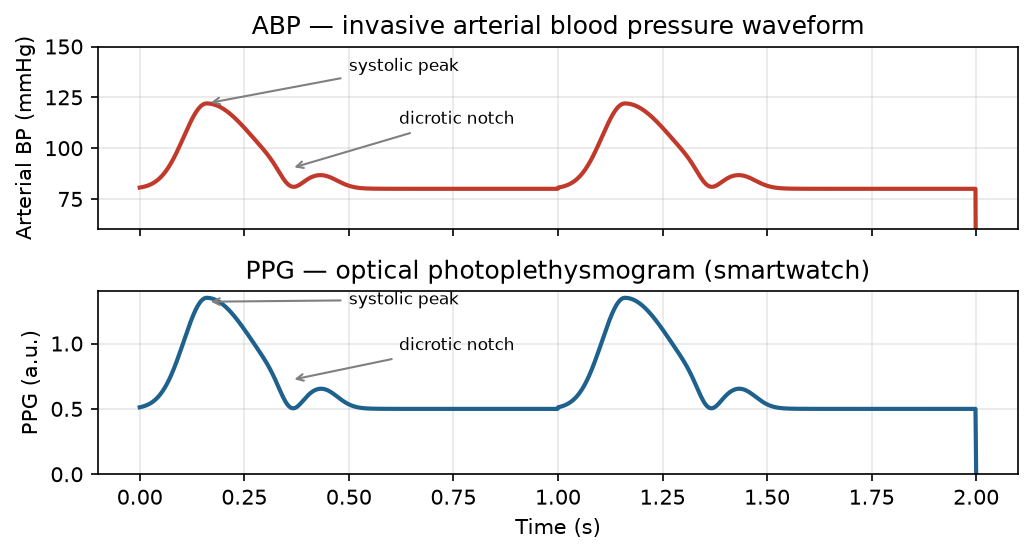
\includegraphics[width=0.78\textwidth]{figures/fig_abp_ppg.png}
\caption{Comparison of the invasive arterial blood pressure (ABP) waveform and the optical photoplethysmogram (PPG). Both signals contain a systolic peak, a dicrotic notch, and a diastolic phase, sharing cardiac morphology despite different sensing principles.}
\label{fig:abp_ppg}
\end{figure}

Systematic feature extraction from the PPG waveform has been studied extensively. Elgendi provides a unified framework for detecting systolic peaks, the dicrotic notch, and the first and second derivatives --- the velocity plethysmogram (VPG) and acceleration plethysmogram (APG) \citep{elgendi2012}. The APG a--e wave amplitudes and their ratios (b/a, c/a, d/a, e/a) are of particular importance: the b/a ratio correlates with vascular resistance and ageing, and the augmentation index (AIx) correlates with arterial stiffness \citep{elgendi2012}. These established biomarkers motivate the 55-dimensional feature set used in this thesis.

\section{Cuffless Blood Pressure Estimation}

Cuffless BP estimation aims to derive BP from continuously available physiological signals. Existing approaches fall into two broad families.

Physiology-driven methods exploit the relationship between pulse wave velocity and arterial stiffness. The pulse transit time (PTT) --- the delay between the ECG R-peak and the PPG systolic peak --- is inversely related to BP through the Moens--Korteweg equation, and has been the basis of extensive research on ubiquitous BP monitoring \citep{mukkamala2015}. PTT-based methods, however, require two sensors and frequent individual recalibration, which limits their practicality. A related approach uses the smartphone camera and finger-pressing to estimate BP from the oscillometric principle \citep{chandrasekhar2018}.

Data-driven methods learn a mapping from PPG features to BP using regression models or neural networks. Classical machine-learning pipelines extract hand-crafted morphological features and train models such as support vector machines or gradient-boosted trees \citep{kachuee2017}. Deep-learning pipelines learn representations directly from raw or spectro-temporal PPG signals; Slapni\v{c}ar et al.\ trained a spectro-temporal convolutional network for BP regression \citep{slapnicar2019}, and Reiss et al.\ demonstrated large-scale heart-rate estimation from PPG with convolutional networks \citep{deepppg2019}. Public datasets such as the MIMIC-III matched waveform subset, VitalDB, and the subsequently derived PulseDB have enabled standardised benchmarking of these methods \citep{mimic2016,vitaldb2022,pulsedb2023}.

Despite steady progress, data-driven methods consistently degrade under cross-subject evaluation: a model trained on a population and tested on unseen subjects typically performs far worse than within-subject evaluation \citep{kachuee2017}. This cross-subject generalisation gap --- the central obstacle addressed in this thesis --- arises because the relationship between PPG morphology and BP varies substantially across individuals owing to differences in vascular elasticity, peripheral resistance, and cardiac output.

\section{Large Language Models}

Large language models (LLMs), built on the Transformer architecture \citep{vaswani2017}, are pre-trained on vast text corpora and exhibit strong in-context learning: given a few labelled examples in the prompt, they adapt to a task at inference time without any parameter update \citep{brown2020}. This capability is attractive for personalisation, because a single pre-trained model can adapt to an individual without fine-tuning.

Recent work has begun to apply LLMs to physiological signals. Health-LLM evaluates the ability of LLMs to make health predictions from wearable sensor data and contextual information, showing that few-shot prompting can ground non-linguistic physiological data \citep{healthllm2024}. Large language models have also been applied directly to cuffless BP measurement from wearable biosignals, demonstrating that textual representations of physiological features enable LLM-based BP regression \citep{llmbp2024}. The few-shot health learning paradigm further shows that LLMs can ground physiological and behavioural time-series data for clinical and wellness tasks \citep{fewshothealth2023}. These results motivate the core hypothesis of this thesis: an LLM can serve as a personalised BP estimator through in-context calibration.

\section{SensorLM: Sensor--Language Alignment}

SensorLM translates wearable sensor data into natural language through hierarchical captions at three levels --- statistical, structural, and semantic --- and pre-trains a family of sensor--language foundation models on large-scale wearable data \citep{sensorlm2025}. Its key insight is that sensor data can be translated into language, providing a bridge through which LLMs can understand and reason about physiological signals, with demonstrated capabilities in zero-shot recognition and few-shot learning.

\section{TimeSRL: Semantic Bottleneck}

TimeSRL abstracts raw time-series data into natural-language descriptions and then makes predictions exclusively from those descriptions, showing that a semantic bottleneck can improve cross-dataset generalisation in behavioural time-series modelling \citep{timesrl2026}. Its finding is directly relevant to this thesis: language can distill the physiological essence of a signal. However, TimeSRL targets classification-style behavioural outcomes, and this thesis shows that for precise regression tasks, purely qualitative abstraction loses critical quantitative information --- a boundary that semantic description must respect by retaining quantitative anchors.

\section{Implications for This Thesis}

These two lines of work illuminate the potential and the boundary of sensor verbalisation: language can highlight physiological essence, but the manner of abstraction is crucial. They form the theoretical foundation of the semantic description approach presented in Chapter~\ref{ch:methodology}, which combines clinical language with quantitative anchors and applies it to personalised BP estimation.
